\section{Przeprowadzone eksperymenty} \label{results}


\subsection{Sztuczne powiekszanie zbioru danych}
\subsubsection{Opis problemu}
Eksperyment sztucznego powiększania danych został przeprowadzony w opraciu o konkurs ,,Dogs vs. Cats'' opublikowanego w serwisie Kaggle.\footnotemark Zadaniem uczestników było stworzenie systemu, który jest w stanie rozwiązać problem rozpoznawania psów i kotów na obrazie. Udostępnione zostało baza danych 25000 sklasyfikowanych obrazów. Mały wycinek udostępnionych danych został przedstawiony na rysunku \ref{catsdogs}. W celu ewaluacji i otrzymania wyniku wykorzystywany był zbiór 12500 niesklasyfikowanych obrazów. Najlepsze rezultaty uczestnicy otrzymywali przy użyciu głębokich sieci neuronów i także ta metoda została wykorzystana w tej pracy.Zwyciezca pierwszej edycji konkursu uzyskal skutecznosc 98,9\%\footnotemark korzystajac wlasnie z glebokich sieci neuronowych.Celem tego eksperymentu było zbadania poprawy klasyfikacji przy użyciu sztucznego powielania danych. Najprosciej ujmujac, cale postepowanie mozna opisac w dwoch krokach. Pierwszym z nich jest uczenie przy uzyciu oryginalnych obrazow. Drugim natomiast, uczenie przy wykorzystywaniu lekko zmodyfikowanych obrazow. W kroku drugim jednak, mozna rowniez wyszczegolnic dwa podejscia:
\begin{itemize}
\item statyczne powielanie obrazow,
\item dynamiczne powielanie obrazow.
\end{itemize}
Stayczne generowanie obrazow polega na stworzeniu ich przed uruchomieniem programu. Mozna okreslic liczbe obrazow, ktore chcemy stworzyc dla kazdego obrazu oryginalnego, nastepnie wygenerowac docelowe obrazy aby ostatecznie uzyc ich do uczenia sieci neuronowej. W przypadku dynamicznego generowanie obrazow, jest ono wykonywane w trakcie dzialania programu za kazdym razem gdy siec potrzebuje danych. Przy uwzglednieniu wystarczajacej ilosci zmiennych losowych zapewnia to, ze z bardzo duzym prawdopodbienstwem nie zostana wykorzystane do uczenia dokladnie dwa takie same obrazy.
\footnotetext{\url{https://www.kaggle.com/c/dogs-vs-cats}}
\footnotetext{\url{https://plus.google.com/+PierreSermanet/posts/GxZHEH9ynoj}}

\begin{figure}[ht!]
\centering
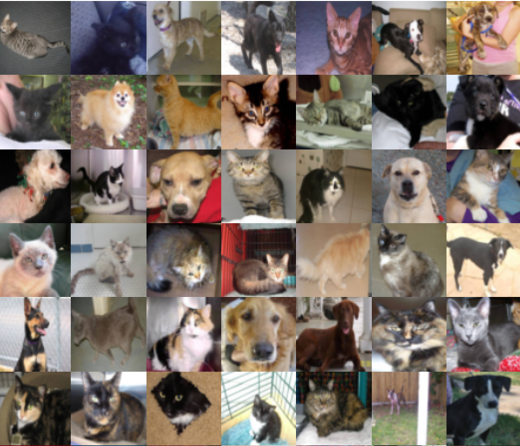
\includegraphics[scale=0.8]{res/catsdogs.png}
\caption[Caption for LOF]{Przykładowe zdjęcia z bazy danych serwisu Kaggle dla konkursu ,,Dogs vs. Cats'' \label{catsdogs}}
\end{figure} 

\subsubsection{Stworzony system}
System stworzony w przypadku tego eksperymentu skladal sie z kilku komponentow. W celu wyodrebnienia wczytywania oraz generowania danych stworzony zostal komponent nazwany DataProvider, ktory pozwalal w zreczny sposob podawac dane do sieci. Glownym komponentem byla sama siec neuronowa. Ze wzgkedy hedbaj ba duze wymogi obliczeniowe w przypadku uczenia, mozliwosci dobrania odpowiedniej architektury oraz optymalizowania parametrow byly dosc ograniczone. Samo uczenie sieci trwalo tyle a tyle godzin.
\subsubsection{Wyniki}
\subsubsection{Wnioski}

\subsection{Walidacja krzyżowa}
\subsubsection{Opis problemu}
\subsubsection{Wyniki}
\subsubsection{Wnioski}

\subsection{Ekstrakcja cech przy użyciu metod matematycznych}
\subsubsection{Opis problemu}
\subsubsection{Stworzony system}
\subsubsection{Wyniki}
\subsubsection{Wnioski}

\subsection{Ekstrakcja cech przy użyciu ,,wiedzy''}
\subsubsection{Opis problemu}
\subsubsection{Stworzony system}
\subsubsection{Wyniki}
\subsubsection{Wnioski}

